\section{Estructuras condicionales: "Por que las lineas son fomes" }

Hasta ahora, con lo que sabemos de python podemos representar todos los digramas de flujo que tienen solo 1 camino en python, como los de a continuacion:

  \begin{center}
    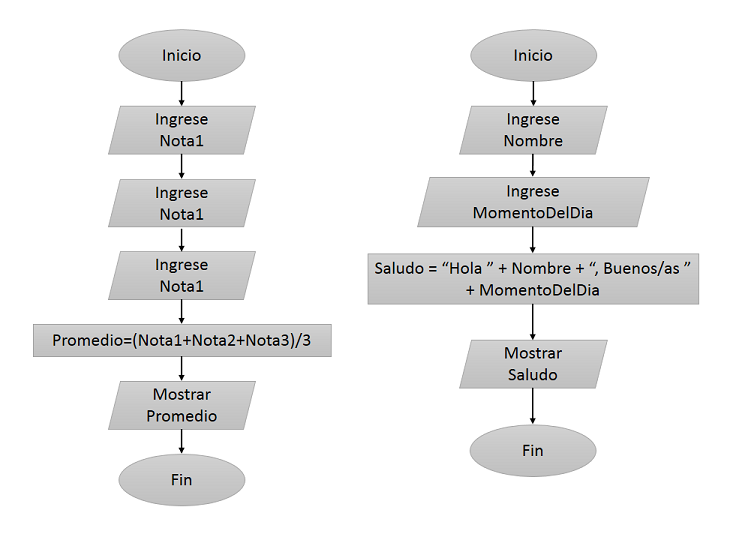
\includegraphics[scale=0.6]{Imagenes/DiagramasFlujo}
  \end{center}
  
Te podras fijar que no es posible con lo que sabemos hasta ahora generare decisiones, es decir, que el programa nos diga si el promedio de las notas es suficiente para pasar el ramo (Ej: $n >55$) o que automaticamente sepa si elegir "Buenos" o "Buenas" para el caso de Tardes, Dias y Noches.

Esto lo solucionamos gracias a las Estructuras Condicionales, o por como ya debes conocerlas en los diagramas de flujos, los rombos.

  \begin{center}
    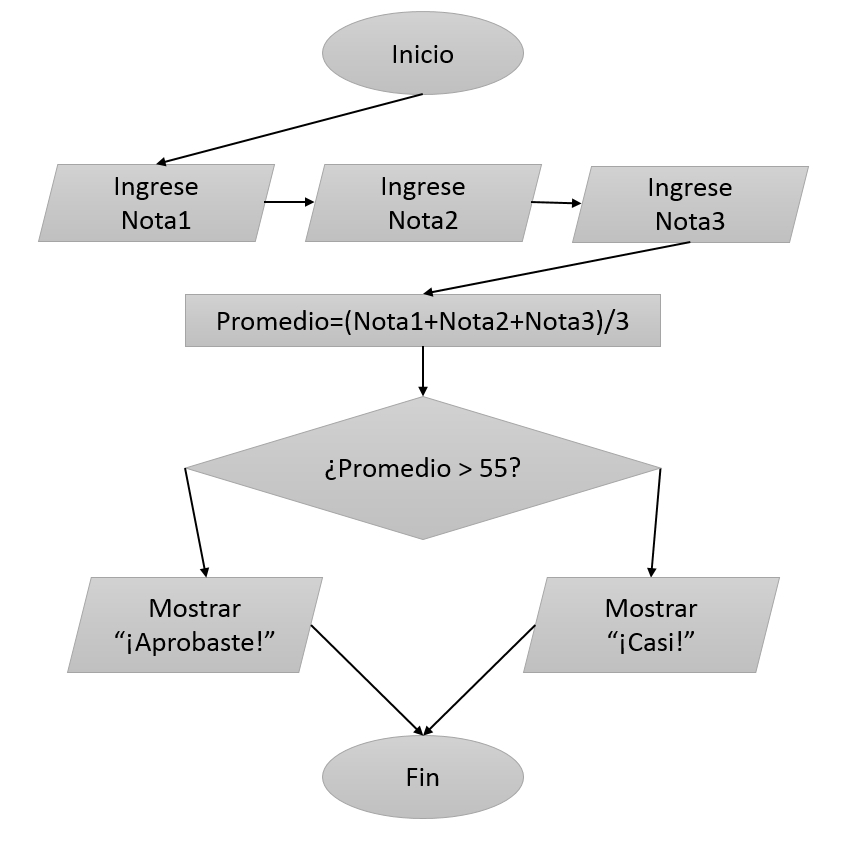
\includegraphics[scale=0.4]{Imagenes/DiagramasFlujo2}
  \end{center}

En  \texttt{python}, los rombos los conoceremos como estructuras condicionales, o bloques \texttt{IF} y los usaremos de la siguiente manera:
 
\lstinputlisting[
    style  = mypy,
    caption= \texttt{EstructurasCondicionales.py}]{Resumen/1.py}

    
Hay que tener en cuenta de que al tener dos \texttt{if} en el mismo nivel, puede suceder el caso de que ocurran simultaneamente, esto se soluciona con ell uso de
\texttt{elif}. Una forma de leerlo en lenguaje natural seria: ``Si esto ocurre, haz esto, y si esto otro ocurre, haz esto otro'' (aqui podrian pasar ambas cosas
a la vez), ahora con \texttt{elif} seria: ``Si esto ocurre haz esto, si no, vee si esto otro ocurre, entonces haz esto otro''.

Ahora, pasando el ejemplo anterior en diagrama de flujo a codigo python (el promedio de los certamenes):

\lstinputlisting[
    style  = mypy,
    caption= \texttt{EstructurasCondicionales.py}]{Resumen/2.py}



